\section*{Solving the equations using Matlab}
\hspace{\parindent}As mentioned before our aim is to solve the equations of the second “real model” and to find the voltage distribution and field intensity everywhere, and of course, to find the velocity of air of the unit we aim to model, so we tried to solve it using Matlab packages and its numerical methods.
\subsection*{The flow of the algorithm}
The flow can be described as follows:
\begin{enumerate}
    \item Defining the parameters we need most important that were mentioned before like permittivity and geometry parameters
    \item Setting the boundary conditions of the second model, as we use the numerical method of (finite difference) to solve all the equations together
    \item  Identifying the grid and mesh
    \item Starting with the initial condition to solve Poisson getting the voltage everywhere
    \item Entering a loop to get better accuracy
    \item Calculating electric field created on the ions
    \item Calculating the velocity to be able to calculate the thrust ("but at this point it was a little hard to get good results at Matlab")
\end{enumerate}
\begin{figure}[ht]
	\centering
	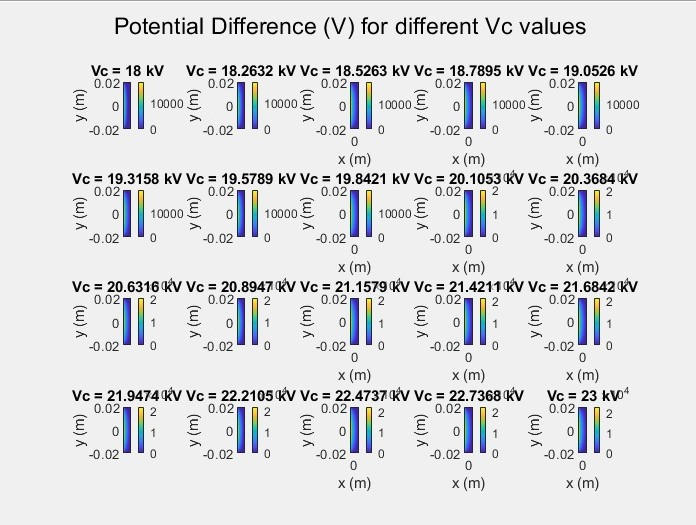
\includegraphics[scale=0.8]{images/results images/matlab images/potential Difference.jpeg}
	\caption{Potential Difference for different applied voltages}
        \vspace*{\floatsep}
        
        	\centering
        	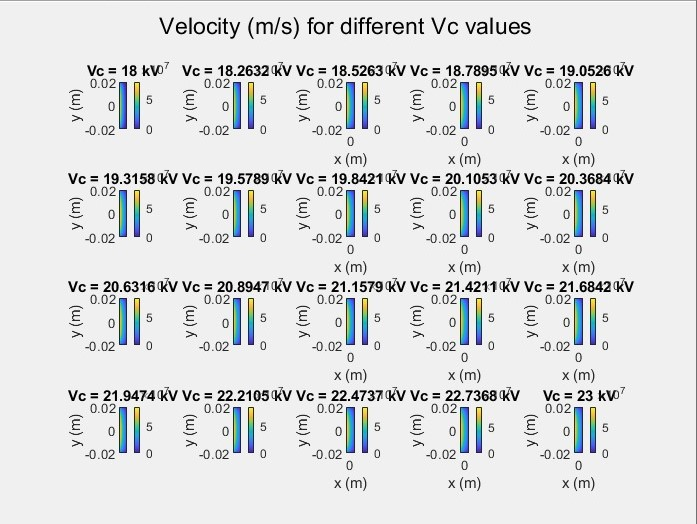
\includegraphics[scale=0.8]{images/results images/matlab images/velocity (2).jpeg}
        	\caption{Velocity intensity for different applied voltages }
        \end{figure}
        